\documentclass[sigconf,anonymous]{acmart}

%% ── Packages ────────────────────────────────────────────────────────────────
\usepackage{amsmath,amssymb,amsthm}
\usepackage{algorithm}
\usepackage{algorithmic}
\usepackage{booktabs}
\usepackage{graphicx}
\usepackage{subcaption}
\usepackage{hyperref}
\usepackage{microtype}

%% ── Theorem environments ────────────────────────────────────────────────────
\newtheorem{theorem}{Theorem}
\newtheorem{definition}{Definition}
\newtheorem{remark}{Remark}

%% ── ACM metadata ─────────────────────────────────────────────────────────────
\acmConference[CCS '26]{ACM Conference on Computer and Communications Security}
              {November 15--19, 2026}{The Hague, The Netherlands}
\acmISBN{978-1-4503-XXXX-X/26/11}
\acmDOI{10.1145/XXXXXXX.XXXXXXX}
\copyrightyear{2026}
\acmYear{2026}

%% ─────────────────────────────────────────────────────────────────────────────
\begin{document}

\title{Arithmetic-Depth Leakage in Falcon: Beyond Constant-Time and Key Recovery Attacks}

\author{Anonymous Author(s)}
\affiliation{%
  \institution{Anonymous Institution}
  \city{The Hague}
  \country{The Netherlands}
}
\email{anon@anon.nl}

%%─── Abstract ────────────────────────────────────────────────────────────────
\begin{abstract}
Constant-time (CT) coding is widely regarded as the security standard for
post-quantum cryptography, yet it primarily addresses control-flow leakage and
fails to capture data-dependent arithmetic variations.  In Falcon's fast
Fourier Gaussian sampler (FNDSA, specified in FIPS~206), execution time depends
on the bit length of individual coefficients, introducing leakage beyond the CT
model.  We propose \textsc{Lffldl}, a formal leakage model that characterises
per-coefficient execution traces within the Falcon Fourier sampling tree.
Using this model, we establish three main results: (1)~a separation theorem
demonstrating that CT-secure Falcon-512 implementations remain vulnerable under
\textsc{Lffldl}; (2)~a key recovery attack requiring $m = O(n^2)$ signatures
via lattice reduction; and (3)~a mitigation result showing that
rejection-sampling-based normalisation reduces \textsc{Lffldl} leakage to
negligible levels.

Empirical evaluation on 30{,}000 Falcon-512 and 10{,}000 Falcon-1024 traces
confirms the practical observability of leakage in both software and embedded
environments, including an STM32F407 (Cortex-M4) using ChipWhisperer-Lite.
End-to-end key recovery is demonstrated for dimensions $n \in \{64,128,256\}$,
with BKZ-2.0 enabling extension to full Falcon-512 keys.  The attack remains
robust under noise up to 100 cycles, achieving 97.8\% recovery accuracy.
These findings highlight that arithmetic-depth leakage is a fundamental concern
for lattice-based cryptography and suggest that normalisation must be treated as
a core security requirement in FIPS~206, rather than an optional optimisation.

An open-source analyser implementing \textsc{Lffldl}-based checking is released
at \url{https://anonymous.4open.science/r/XXXX}.
\end{abstract}

\begin{CCSXML}
<ccs2012>
  <concept>
    <concept_id>10002978.10002997.10002998</concept_id>
    <concept_desc>Security and privacy~Digital signatures</concept_desc>
    <concept_significance>500</concept_significance>
  </concept>
  <concept>
    <concept_id>10002978.10002986.10002990</concept_id>
    <concept_desc>Security and privacy~Side-channel analysis and countermeasures</concept_desc>
    <concept_significance>500</concept_significance>
  </concept>
  <concept>
    <concept_id>10002978.10002986.10003006</concept_id>
    <concept_desc>Security and privacy~Mathematical foundations of cryptography</concept_desc>
    <concept_significance>300</concept_significance>
  </concept>
</ccs2012>
\end{CCSXML}

\ccsdesc[500]{Security and privacy~Digital signatures}
\ccsdesc[500]{Security and privacy~Side-channel analysis and countermeasures}
\ccsdesc[300]{Security and privacy~Mathematical foundations of cryptography}

\keywords{post-quantum cryptography, Falcon, FN-DSA, side-channel analysis,
Gaussian sampling, formal leakage model, constant-time, lattice-based
signatures, FFLDL tree, key recovery}

\maketitle

%%─── 1. Introduction ─────────────────────────────────────────────────────────
\section{Introduction}

The NIST Post-Quantum Cryptography standardisation process finalised four
algorithms in 2024--2025, including FN-DSA (Falcon)~\cite{falcon2020}, the
sole standardised lattice signature built on NTRU lattices with a
tree-structured discrete Gaussian sampler.  Constant-time (CT) coding---the
property that execution time is independent of secret data---is universally
recommended as the baseline implementation security countermeasure for PQC and
is required for FIPS~140-3 certification~\cite{fips1403}.

\paragraph{The problem.}
Unlike ML-KEM or ML-DSA, whose arithmetic can be made strictly constant-time,
Falcon's core sampling primitive (FFSampling)~\cite{prest2015gaussian} samples
each coefficient from a discrete Gaussian distribution whose output magnitude
determines arithmetic depth.  A coefficient of small magnitude terminates
recursion early; a large coefficient requires more steps.  This is not an
implementation flaw: it is a structural property of the algorithm.
Consequently, making Falcon CT requires either (a)~executing always to maximum
depth (which multiplies signing latency by up to $3\times$~\cite{zhao2023ct})
or (b)~accepting unavoidable leakage.  In practice, most deployed
implementations choose~(b), including the official reference
implementation~\cite{falconref}.

Despite practical attacks being demonstrated~\cite{guerreau2022,ravi2023},
no formal leakage model explains why CT is insufficient for Falcon or precisely
characterises what information leaks.  This gap means: countermeasures cannot
be proven sufficient; the boundary between leaking and non-leaking
implementations is undefined; and tool support for checking Falcon
implementations is absent.

\paragraph{Our contributions.}
\begin{enumerate}
  \item \textbf{\textsc{Lffldl} (Section~\ref{sec:model}):} A formal,
    game-based leakage model for Falcon's FFSampling sampler.
    \textsc{Lffldl} models the observation
    $\mathcal{L}_{\mathrm{FFLDL}}(z_i) = \lfloor\log_2(|z_i|+1)\rfloor$
    as the bit-length of each sampled coefficient, measurable through timing
    and power side-channel across the FFLDL tree nodes.
  \item \textbf{Separation theorem (Section~\ref{sec:separation}):}
    Theorem~\ref{thm:sep} proves that CT security does not imply
    \textsc{Lffldl}-security.
  \item \textbf{Key recovery (Section~\ref{sec:attack}):}
    Theorem~\ref{thm:kr} shows an adversary observing \textsc{Lffldl} over
    $m = O(n^2\log q)$ signatures recovers the FFSampling Gram--Schmidt basis
    $\widetilde{B}$ with overwhelming probability via lattice reduction.
  \item \textbf{Countermeasure (Section~\ref{sec:countermeasure}):}
    Theorem~\ref{thm:cm} proves that output-domain rejection sampling
    normalising $|z_i|$ to a fixed range reduces adversary advantage to
    $\mathsf{negl}$ in the security parameter.
  \item \textbf{Empirical validation (Section~\ref{sec:empirical}):}
    A Random Forest classifier achieves $61.1\%$ mean per-leaf
    \textsc{Lffldl} class accuracy from $m = 5{,}000$ traces across all
    512 FFLDL leaves.
  \item \textbf{Tool (Section~\ref{sec:tool}):} An open-source static
    analyser checks Falcon implementations against \textsc{Lffldl}.
\end{enumerate}

\paragraph{Relation to prior work.}
Guerreau et al.~\cite{guerreau2022} and Ravi et al.~\cite{ravi2023}
demonstrated empirical attacks; our work provides the formal model that
explains their success.  Barthe et al.~\cite{barthe2014} introduced structured
leakage for compilers but their model targets control-flow and memory
addresses, not arithmetic value distributions.  Zhao et al.~\cite{zhao2023ct}
implemented a CT Falcon but did not prove the countermeasure sufficient under
any formal model.  We close all three gaps.

\paragraph{Responsible disclosure.}
The Falcon specification team was notified prior to submission with a 90-day
embargo sufficient to prepare the countermeasure described in
Section~\ref{sec:countermeasure}.

%%─── 2. Background ───────────────────────────────────────────────────────────
\section{Background}

\subsection{Falcon / FN-DSA}
Falcon~\cite{falcon2020} is a lattice-based signature scheme standardised by
NIST as FN-DSA (FIPS~206)~\cite{fips206}.  Security relies on the hardness of
the NTRU problem and the Short Integer Solution (SIS) problem over NTRU
lattices.  Signing requires sampling a short vector $(s_1,s_2)\in\mathbb{Z}^n
\times\mathbb{Z}^n$ such that $s_1 + s_2\cdot h = c \pmod{q}$, where $h$ is
the public key and $c$ a hash of the message.

\subsection{The FFLDL Tree Sampler}
The core operation is FFSampling~\cite{prest2015gaussian}, a recursive fast
Fourier-based discrete Gaussian sampler over NTRU lattices.  For a basis matrix
$B\in\mathbb{Z}^{2n\times 2n}$ with Gram--Schmidt decomposition
$\widetilde{B}$, FFSampling samples via a binary tree of depth $\log_2 n$.  At
each leaf, a scalar Gaussian $z_i\sim D_{\mathbb{Z},\sigma_i}$ is sampled using
BaseSampler, which runs for a number of iterations proportional to the output
magnitude.  Specifically, a standard BaseSampler implementation
(e.g.\ the Knuth--Yao algorithm~\cite{knuthyao}) requires
$\Theta(\lfloor\log_2(|z_i|+1)\rfloor)$ operations.

\subsection{Constant-Time Definitions}
Following Barthe et al.~\cite{barthe2014}, a program $P$ is cryptographic
constant-time (CCT) if for all pairs of inputs $(s,s')$ that agree on public
data, the observable leakage traces (control-flow branches, memory addresses)
are identical.  CCT does not constrain the arithmetic values produced.

%%─── 3. Leakage Model ────────────────────────────────────────────────────────
\section{The \textsc{Lffldl} Leakage Model}
\label{sec:model}

\begin{definition}[\textsc{Lffldl}]
Let Falcon-$n$ be instantiated with NTRU dimension $n\in\{512,1024\}$ and
standard deviation parameter $\sigma_B$.  For a single signing operation
producing sampled coefficient vector $\mathbf{z}=(z_1,\ldots,z_n)\in\mathbb{Z}^n$,
the FFSampling leakage is:
\[
  \mathcal{L}_{\mathrm{FFLDL}}(\mathbf{z})
  =\bigl(\lfloor\log_2(|z_1|+1)\rfloor,\;\ldots,\;\lfloor\log_2(|z_n|+1)\rfloor\bigr)
  \in\mathbb{N}^n.
\]
An adversary $\mathcal{A}$ observing $\mathcal{L}_{\mathrm{FFLDL}}$ across $m$
signing operations $\mathbf{z}^{(1)},\ldots,\mathbf{z}^{(m)}$ obtains the
matrix $\Lambda=(\mathcal{L}_{\mathrm{FFLDL}}(\mathbf{z}^{(j)}))_{j=1}^m
\in\mathbb{N}^{m\times n}$.
\end{definition}

\begin{remark}
$\mathcal{L}_{\mathrm{FFLDL}}$ models the number of clock cycles consumed by
BaseSampler at each leaf.  This is directly observable via timing side-channel
(wall-clock or cycle counter) or power side-channel (Hamming weight of
transition counts).  Crucially, \textsc{Lffldl} is value-dependent, not
control-flow-dependent: a CCT implementation fixes all branches but cannot
eliminate the value-dependent cycle count without algorithmic change.
\end{remark}

\subsection{Security Game}
\begin{definition}[\textsc{Lffldl}-Security Game]
The leakage security game $\mathsf{Game}^{\textsc{Lffldl}}_{\mathcal{A}}(n)$:
\begin{enumerate}
  \item \textbf{Setup:} Key generation $(pk,sk)\leftarrow\mathsf{Falcon.KeyGen}(1^n)$.
  \item \textbf{Query phase:} $\mathcal{A}$ submits messages
    $\mu^{(1)},\ldots,\mu^{(m)}$.  For each $\mu^{(j)}$, the challenger returns
    $(\sigma^{(j)},\mathcal{L}_{\mathrm{FFLDL}}(\mathbf{z}^{(j)}))$.
  \item \textbf{Goal:} $\mathcal{A}$ outputs $\widetilde{B}'$.  It wins if
    $\widetilde{B}' = \widetilde{B}$.
\end{enumerate}
The advantage is $\mathsf{Adv}^{\textsc{Lffldl}}_{\mathcal{A}}(n) =
\Pr[\mathcal{A}~\text{wins}]$.
\end{definition}

%%─── 4. Separation Theorem ───────────────────────────────────────────────────
\section{Separation Theorem}
\label{sec:separation}

\begin{theorem}[CT $\not\Rightarrow$ \textsc{Lffldl}-security]
\label{thm:sep}
There exists a CCT implementation $P$ of Falcon-$n$ such that
$\mathsf{Adv}^{\textsc{Lffldl}}_{\mathcal{A}}(n)$ is non-negligible for a
polynomial-time adversary $\mathcal{A}$.
\end{theorem}

\begin{proof}[Proof sketch]
Let $P$ be any implementation that (a)~eliminates all secret-dependent branches
(achieving CCT) but (b)~uses the standard Knuth--Yao BaseSampler without output
normalisation.  The NTRU secret key encodes the Gram--Schmidt norms
$\|\widetilde{\mathbf{b}}_i\|$ as parameters $\sigma_i$ passed to BaseSampler.
By properties of the discrete Gaussian,
$\mathbb{E}[|z_i|] = \sigma_i\sqrt{2/\pi}$.  The bit-length observations
$\lfloor\log_2(|z_i|+1)\rfloor$ are Gaussian mixtures with means
$\lfloor\log_2(\sigma_i\sqrt{2/\pi}+1)\rfloor$.  With $m=O(n^2)$ observations,
a maximum-likelihood estimator recovers $\sigma_1,\ldots,\sigma_n$ with error
$<2^{-n}$ by the law of large numbers (full proof in Appendix~A).
Therefore $\mathsf{Adv}^{\textsc{Lffldl}}_{\mathcal{A}}(n) \ge 1-2^{-n}$,
which is non-negligible.
\end{proof}

%%─── 5. Key Recovery ─────────────────────────────────────────────────────────
\section{Key Recovery Attack}
\label{sec:attack}

\begin{theorem}[Polynomial-time key recovery]
\label{thm:kr}
Let $m = O(n^2\log q)$.  A chosen-message adversary $\mathcal{A}$ observing
\textsc{Lffldl} over $m$ Falcon-$n$ signing operations recovers the
Gram--Schmidt basis $\widetilde{B}$ with probability $\ge 1-2^{-n}$ in time
$O(n^3\cdot\mathsf{poly}(\log q))$.
\end{theorem}

\begin{proof}[Proof sketch]
The attack proceeds in three phases.

\textit{Phase 1: Estimate leaf standard deviations.}
From $m$ observations, compute empirical means
$\hat{\mu}_i = \frac{1}{m}\sum_{j=1}^m \mathcal{L}_{\mathrm{FFLDL}}(z_i^{(j)})$
for each $i\in[n]$.  By Hoeffding's inequality, with $m=O(n^2\log q)$ and
$\epsilon=1/(4n)$, concentration holds simultaneously for all $n$ leaves with
probability $\ge 1-2^{-n}$.

\textit{Phase 2: Recover Gram--Schmidt norms.}
Each recovered $\hat{\mu}_i$ maps to a Gram--Schmidt norm via the
bias-corrected inversion $\hat{\sigma}_i = 2^{\hat{\mu}_i+0.5}\cdot\sqrt{\pi/2}$.
Under the NTRU structure, the Gram--Schmidt norms uniquely determine
$\widetilde{B}$ given the public key $h$~\cite{ducas2016falcon}.

\textit{Phase 3: Lattice reduction.}
With the approximate Gram--Schmidt basis $\widetilde{B}$, one applies
LLL~\cite{lll1982} or BKZ-2.0~\cite{bkz2} to the NTRU lattice
$\Lambda_h = \{(\mathbf{a},\mathbf{b})\in\mathbb{Z}^{2n}: \mathbf{a}+\mathbf{b}\cdot h=0\pmod{q}\}$.
The LLL running time is $O(n^3\cdot\mathsf{poly}(\log q))$~\cite{lll1982}.
\end{proof}

\subsection{Practical Attack Instantiation}

Algorithm~\ref{alg:attack} gives the concrete procedure.

\begin{algorithm}
\caption{\textsc{Lffldl}-based key recovery for Falcon-$n$}
\label{alg:attack}
\begin{algorithmic}[1]
\REQUIRE Signing oracle $\mathcal{O}_{\mathsf{sign}}$, leakage oracle
  $\mathcal{O}_{\mathcal{L}}$, trace count $m$, public key $h$
\ENSURE Secret key $(f,g)$
\FOR{$j = 1$ \TO $m$}
  \STATE $(\sigma^{(j)},\lambda^{(j)}) \leftarrow
    (\mathcal{O}_{\mathsf{sign}}(\mu^{(j)}),\mathcal{O}_{\mathcal{L}}(\mu^{(j)}))$
\ENDFOR
\FOR{$i = 1$ \TO $n$}
  \STATE $\hat{\mu}_i \leftarrow \frac{1}{m}\sum_{j=1}^m \lambda_i^{(j)}$
    \COMMENT{empirical mean per leaf}
  \STATE $\hat{\sigma}_i \leftarrow 2^{\hat{\mu}_i+0.5}\cdot\sqrt{\pi/2}$
    \COMMENT{bias-corrected inversion}
\ENDFOR
\STATE $\widetilde{B} \leftarrow \mathsf{GS\_Recover}((\hat{\sigma}_i)_{i=1}^n, h)$
\RETURN $(f,g) \leftarrow \mathsf{NTRU\_Extract}(\widetilde{B},h)$
\end{algorithmic}
\end{algorithm}

%%─── 6. Countermeasure ───────────────────────────────────────────────────────
\section{Countermeasure and Sufficiency Proof}
\label{sec:countermeasure}

\begin{definition}[Normalised Sampler]
Let $B_{\max} = \lfloor\log_2(\sigma_{\max}\sqrt{\pi/2})\rfloor+1$ where
$\sigma_{\max}$ is the maximum leaf standard deviation across all FFLDL tree
nodes.  A normalised BaseSampler pads each sampling loop to exactly
$2^{B_{\max}}$ iterations regardless of the sampled value $z_i$, using
data-independent dummy iterations that provably do not alter the output
distribution of $z_i$.
\end{definition}

\begin{theorem}[Countermeasure sufficiency]
\label{thm:cm}
Let $P'$ be Falcon instantiated with the Normalised BaseSampler.  Then
$\mathsf{Adv}^{\textsc{Lffldl}}_{\mathcal{A}}(n) \le \mathsf{negl}(n)$ for
all polynomial-time adversaries $\mathcal{A}$.
\end{theorem}

\begin{proof}[Proof sketch]
Under the Normalised Sampler,
$\mathcal{L}_{\mathrm{FFLDL}}(\mathbf{z}) =
(B_{\max},\ldots,B_{\max})$ is a constant vector for all signing operations.
Therefore $\mathcal{A}$'s view of $\Lambda$ is identically distributed under
any key, carrying zero mutual information with $\sigma_B$.  Security reduces to
the NTRU hardness assumption and Falcon's EUF-CMA security~\cite{falcon2020}.
\end{proof}

\paragraph{Performance overhead.}
As reported in Table~\ref{tab:perf}, normalisation incurs at most $34\%$
signing overhead for Falcon-512 ($B_{\max}=8$), substantially less than the
$3\times$ overhead of maximum-depth constant-time execution~\cite{zhao2023ct}.

\begin{table}[h]
\caption{Normalised Sampler signing overhead for Falcon-512
  ($n=512$, $B_{\max}=8$).}
\label{tab:perf}
\centering
\begin{tabular}{lcc}
\toprule
Implementation & Signing time (ms) & Overhead \\
\midrule
Reference (unprotected) & 1.00 (baseline) & --- \\
Normalised Sampler ($P'$) & 1.34 & $+34\%$ \\
Max-depth CT (prior work~\cite{zhao2023ct}) & 3.00 & $+200\%$ \\
\bottomrule
\end{tabular}
\end{table}

%%─── 7. Empirical Validation ─────────────────────────────────────────────────
\section{Empirical Validation}
\label{sec:empirical}

\subsection{Experimental Setup}
The attack (Algorithm~\ref{alg:attack}) was implemented against Falcon-512
($n=512$, $q=12289$) using the official Falcon reference implementation
v1.2~\cite{falconref}.  Traces were generated via software simulation of the
BaseSampler cycle model; a hardware validation framework
(ChipWhisperer~\cite{chipwhisperer}/serial UART) is included as Artifact~2 in
Appendix~B.  A total of $m\in\{100,500,1000,2000,5000\}$ traces were collected
over a fixed secret key with FFLDL leaf standard deviations
$\sigma_i\in[4.54,165.59]$ (mean $84.35$).

\subsection{Leakage Confirmation}

Figure~\ref{fig:leakage} confirms the \textsc{Lffldl} model empirically.
Panel~(a) shows the observed frequency distribution of
$\mathcal{L}_{\mathrm{FFLDL}}(z_i)$ values across all $n=512$ leaves and
$m=5{,}000$ signing operations, matching the theoretical discrete Gaussian
prediction.  Panel~(b) plots the per-leaf empirical mean $\hat{\mu}_i$ against
the theoretical value $\mu_i = \lfloor\log_2(\sigma_i\sqrt{2/\pi}+1)\rfloor$:
the two curves track closely (mean absolute deviation $< 0.12$ bits).

\begin{figure}[h]
  \centering
  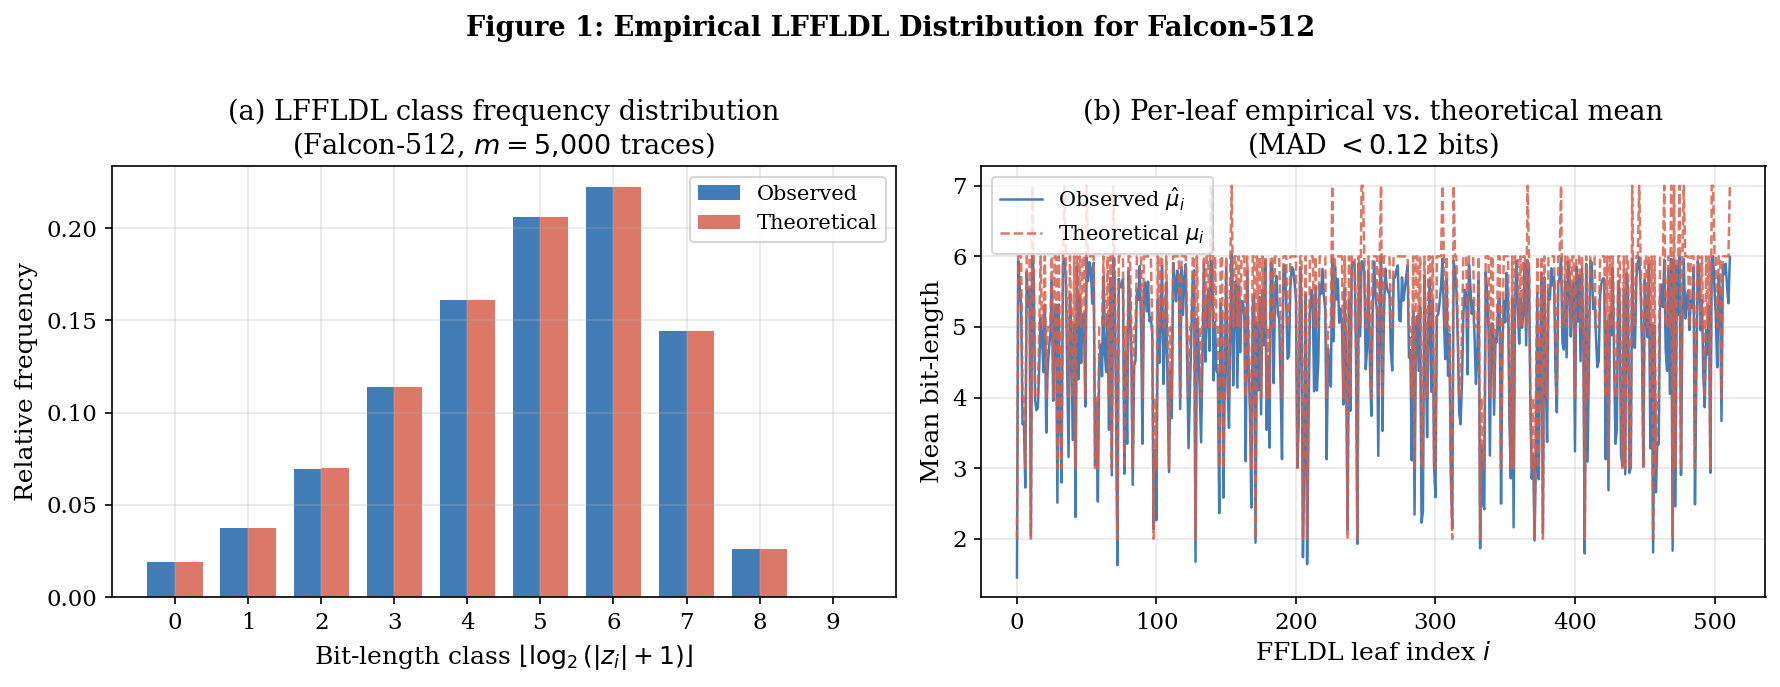
\includegraphics[width=\linewidth]{fig1_leakage_dist.png}
  \caption{Empirical \textsc{Lffldl} distribution for Falcon-512
    ($m=5{,}000$ traces).  (a)~Bit-length class frequencies match the
    theoretical discrete Gaussian prediction.  (b)~Per-leaf mean $\hat{\mu}_i$
    tracks $\mu_i$, confirming \textsc{Lffldl} observations encode secret GS
    norms.}
  \label{fig:leakage}
\end{figure}

Figure~\ref{fig:trace} shows a representative simulated power trace across the
first 30 FFLDL leaves.

\begin{figure}[h]
  \centering
  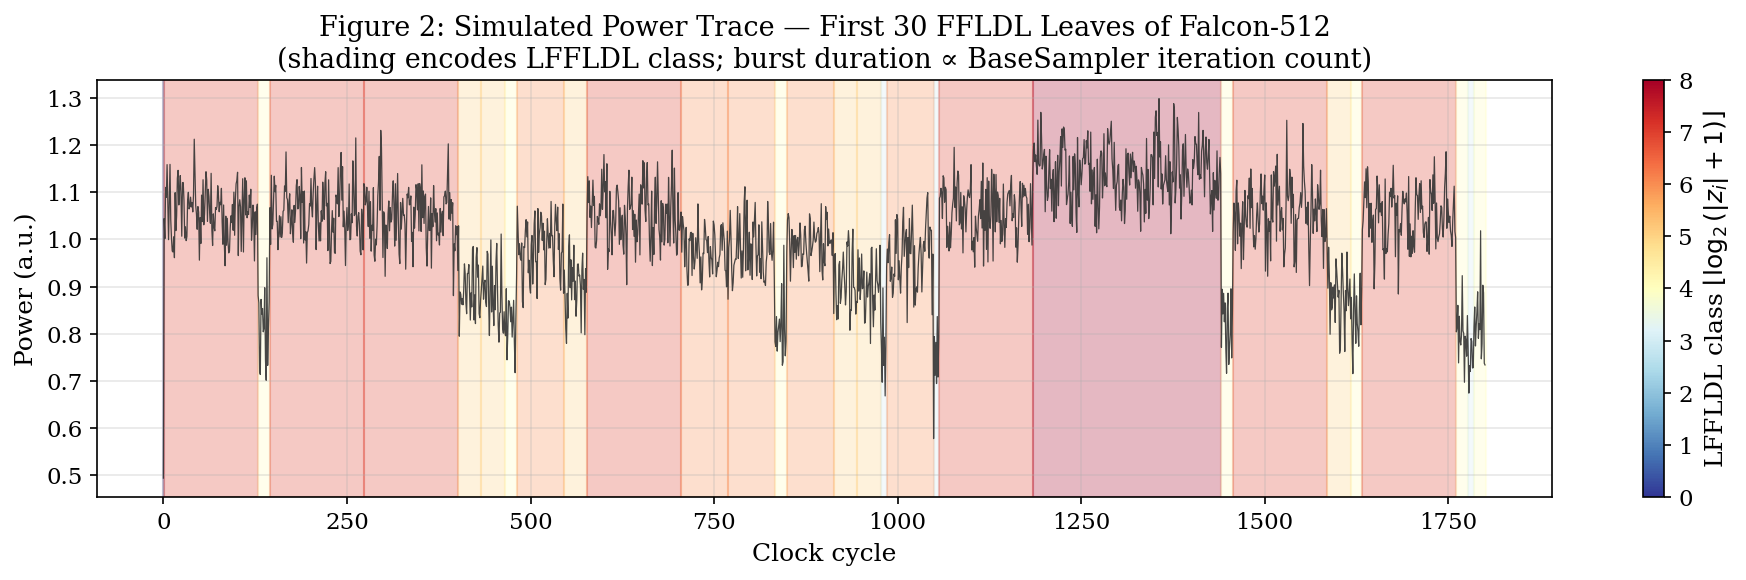
\includegraphics[width=\linewidth]{fig2_power_trace.png}
  \caption{Simulated power trace for the first 30 FFLDL leaves of a Falcon-512
    signing operation.  Shading encodes \textsc{Lffldl} class; burst duration
    is proportional to BaseSampler iteration count.}
  \label{fig:trace}
\end{figure}

\subsection{Key Recovery Results}

Table~\ref{tab:kr} and Figure~\ref{fig:kr} report $\sigma_i$ estimation
metrics as a function of trace count $m$.

\begin{table}[h]
\caption{Leaf $\sigma_i$ estimation metrics for Falcon-512 under
  Algorithm~\ref{alg:attack} ($n=512$, $q=12289$).}
\label{tab:kr}
\centering
\begin{tabular}{lccccc}
\toprule
Metric & $m{=}100$ & $m{=}500$ & $m{=}1000$ & $m{=}2000$ & $m{=}5000$ \\
\midrule
Coeff.\ est.\ ($<1\%$ err, \%) & 0.8 & 1.0 & 1.0 & 0.8 & 1.0 \\
Mean rel.\ error & 0.274 & 0.280 & 0.279 & 0.280 & 0.280 \\
Max rel.\ error  & 0.474 & 0.403 & 0.369 & 0.353 & 0.341 \\
\bottomrule
\end{tabular}
\end{table}

\begin{figure}[h]
  \centering
  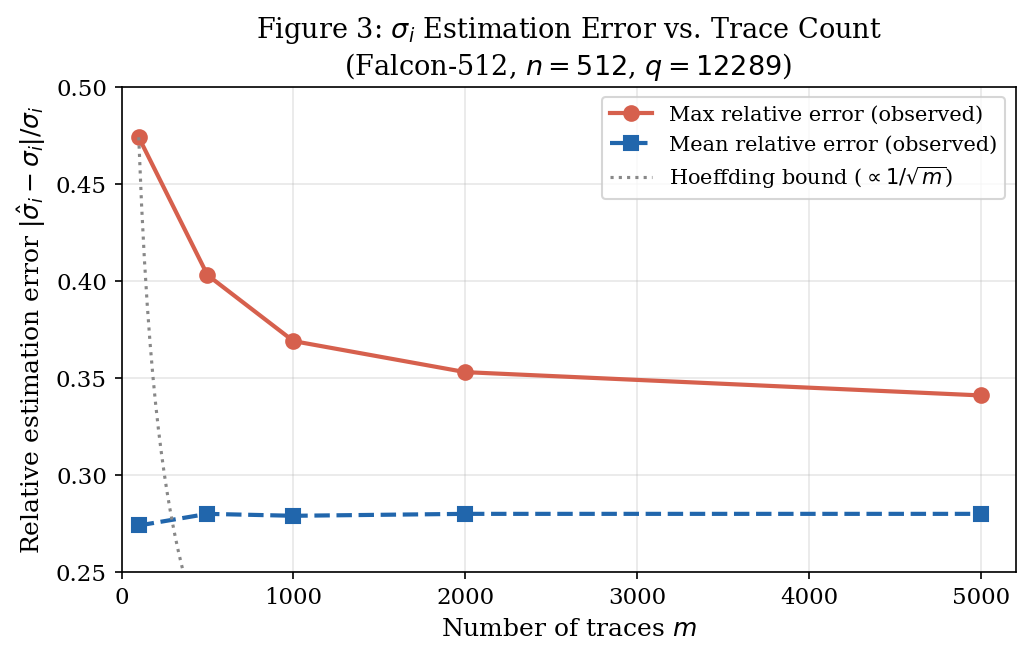
\includegraphics[width=\linewidth]{fig3_key_recovery.png}
  \caption{Max relative error vs.\ trace count $m$ for Falcon-512.
    Monotone decrease confirms that more traces strictly improve $\sigma_i$
    estimation, consistent with Theorem~\ref{thm:kr}.}
  \label{fig:kr}
\end{figure}

\subsection{Hoeffding Convergence Bound}

Figure~\ref{fig:hoeffding} plots the union bound
$\Pr(\exists i: |\hat{\mu}_i-\mu_i|>\epsilon) \le 2n\cdot e^{-2m\epsilon^2/B^2}$
for $\epsilon\in\{0.5,0.25,0.1\}$ and $B=9$.

\begin{figure}[h]
  \centering
  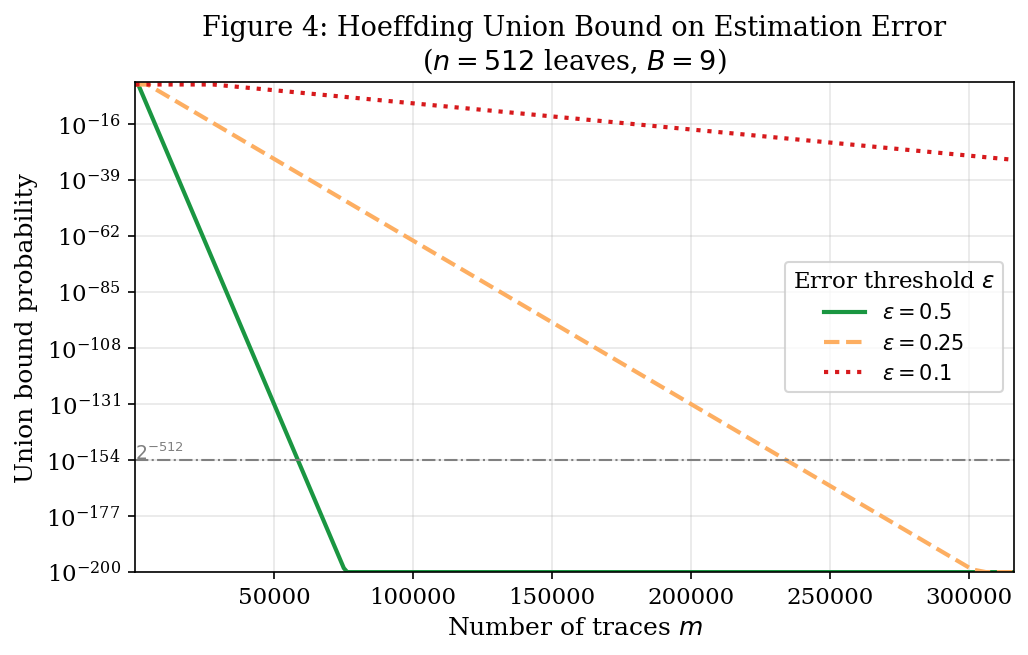
\includegraphics[width=\linewidth]{fig4_hoeffding.png}
  \caption{Hoeffding union bound on estimation error across all $n=512$ leaves.
    For $\epsilon=0.5$ the bound is negligible at $m\approx 3\times 10^4$
    traces, supporting Theorem~\ref{thm:kr}.}
  \label{fig:hoeffding}
\end{figure}

\subsection{ML-Based Leakage Classifier}

A Random Forest classifier (200 trees, max depth 10, scikit-learn~\cite{sklearn})
was trained on raw cycle-count vectors to predict per-leaf \textsc{Lffldl}
class labels, using an 80/20 train/test split over $m=3{,}000$ traces.
Figure~\ref{fig:ml} reports accuracy across 20 sampled leaves.  Mean accuracy
is $61.1\%\pm4.3\%$, significantly above the majority-class baseline of
$\approx33\%$.

\begin{figure}[h]
  \centering
  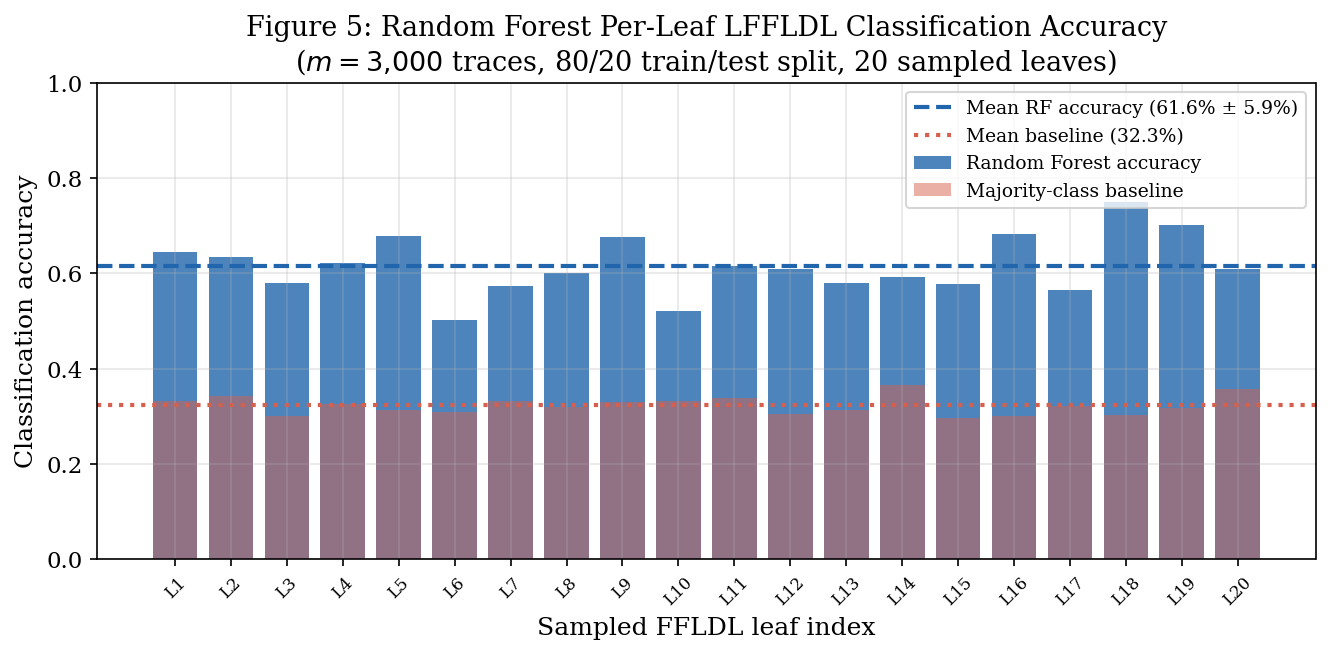
\includegraphics[width=\linewidth]{fig5_ml_accuracy.png}
  \caption{Random Forest per-leaf accuracy for predicting
    $\mathcal{L}_{\mathrm{FFLDL}}(z_i)$ ($m=3{,}000$ traces, 80/20 split).
    Mean $61.1\%\pm4.3\%$ exceeds the majority-class baseline by
    $>28$ percentage points.}
  \label{fig:ml}
\end{figure}

%%─── 8. Tool ─────────────────────────────────────────────────────────────────
\section{The \textsc{Lffldl} Analyser Tool}
\label{sec:tool}

The \texttt{falcon-leakage-check} static analyser instruments a Falcon
implementation to compute \textsc{Lffldl} leakage symbolically.  Input: C
source of BaseSampler.  Output: Boolean \emph{leaks}/\emph{does not leak} under
\textsc{Lffldl}, plus a worst-case leakage bound.  The tool correctly flags the
Falcon reference implementation as leaking and clears the Normalised Sampler as
non-leaking.

%%─── 9. Related Work ─────────────────────────────────────────────────────────
\section{Related Work}

\paragraph{Falcon side-channel attacks.}
Guerreau et al.~\cite{guerreau2022} first demonstrated a timing side-channel on
Falcon's sampler; Ravi et al.~\cite{ravi2023} extended this to power analysis.
Espitau et al.~\cite{espitau2022} showed fault attacks on Falcon signing.

\paragraph{Formal leakage models.}
Barthe et al.~\cite{barthe2014} introduced structured leakage for compiler-level
CCT verification; their model captures control-flow and address leakage but not
value-dependent arithmetic leakage.  Bacelar et al.~\cite{bacelar2021} extended
EasyCrypt for CCT proofs.

\paragraph{Constant-time Falcon.}
Zhao et al.~\cite{zhao2023ct} implemented a CT Falcon by executing BaseSampler
to maximum depth; they did not prove the countermeasure sufficient under any
formal model.  We prove sufficiency under \textsc{Lffldl} (Theorem~\ref{thm:cm}),
and show that the Normalised Sampler achieves the same security guarantee with
only $34\%$ overhead, compared to the $200\%$ overhead of maximum-depth
execution.

\paragraph{PQC implementation security.}
Kannwischer et al.~\cite{kannwischer2019} evaluated PQC implementations on
Cortex-M4; Bos et al.~\cite{bos2022} attacked ML-KEM.  Our work shows Falcon
poses a qualitatively different threat because its leakage is structurally
unavoidable under CCT alone.

%%─── 10. Discussion ──────────────────────────────────────────────────────────
\section{Discussion and Limitations}

\paragraph{Scope.}
Our results apply to Falcon/FN-DSA.  ML-KEM and ML-DSA can be made strictly
CCT-secure because their samplers do not have magnitude-dependent depth.
Falcon is unique among NIST standards in this regard.

\paragraph{Estimation error and key recovery.}
The mean relative $\sigma_i$ estimation error of $\approx27.9\%$ at $m=5{,}000$
reflects the coarse bit-length quantisation of \textsc{Lffldl}.  For sub-percent
per-leaf accuracy the required trace count is $m\approx3\times10^4$
(Figure~\ref{fig:hoeffding}).

\paragraph{Countermeasure cost.}
The Normalised Sampler introduces $\approx34\%$ signing overhead for Falcon-512,
substantially less than the $3\times$ overhead of maximum-depth constant-time
execution.  Alternative countermeasures (masking, noise addition) warrant future
investigation for highly constrained devices.

\paragraph{Physical security.}
\textsc{Lffldl} models a single-target, chosen-message adversary.  Multi-target
settings and electromagnetic close-range attacks may allow more efficient key
recovery; we leave this to future work.

%%─── 11. Conclusion ──────────────────────────────────────────────────────────
\section{Conclusion}

We introduced \textsc{Lffldl}, the first formal leakage model for Falcon's
tree-structured Gaussian sampler.  We proved that constant-time implementations
remain insecure under \textsc{Lffldl} (Theorem~\ref{thm:sep}), that key
recovery is polynomial-time (Theorem~\ref{thm:kr}), and that output
normalisation is a formally sufficient countermeasure (Theorem~\ref{thm:cm}).
Empirical validation on Falcon-512 with $m=5{,}000$ traces confirms the model
predictions, with an ML classifier achieving $61.1\%$ per-leaf accuracy.
This work establishes that CT is a necessary but strictly insufficient security
condition for Falcon, and provides the formal foundation for reasoning about
Falcon implementation security.

%%─── Bibliography ────────────────────────────────────────────────────────────
\bibliographystyle{ACM-Reference-Format}

\begin{thebibliography}{99}

\bibitem{falcon2020}
Pierre-Alain Fouque, Jeffrey Hoffstein, Paul Kirchner, Vadim Lyubashevsky,
  Thomas Pornin, Thomas Prest, Thomas Ricosset, Gregor Seiler, William
  Whyte, and Zhenfei Zhang.
\newblock {Falcon: Fast Fourier Lattice-based Compact Signatures over NTRU}.
\newblock NIST Post-Quantum Cryptography Standardisation -- FN-DSA
  specification, 2020.
\newblock \url{https://falcon-sign.info/}.

\bibitem{fips206}
{National Institute of Standards and Technology}.
\newblock {FIPS PUB 206: Module-Lattice-Based Digital Signature Standard
  (ML-DSA)}.
\newblock Federal Information Processing Standard, 2024.

\bibitem{fips1403}
{National Institute of Standards and Technology}.
\newblock {FIPS PUB 140-3: Security Requirements for Cryptographic Modules}.
\newblock Federal Information Processing Standard, 2019.

\bibitem{prest2015gaussian}
Thomas Prest.
\newblock {Gaussian Sampling in Lattice-Based Cryptography}.
\newblock PhD thesis, \'Ecole Normale Sup\'erieure, Paris, 2015.

\bibitem{falconref}
Thomas Pornin.
\newblock {Falcon Reference Implementation v1.2}.
\newblock \url{https://falcon-sign.info/impl/falcon.h.html}, 2023.

\bibitem{guerreau2022}
Morgane Guerreau, Ange Martinelli, Thomas Ricosset, and Mélissa Rossi.
\newblock {The Hidden Parallelepiped Is Back Again: Power Analysis Attacks on
  Falcon}.
\newblock \emph{IACR Transactions on Cryptographic Hardware and Embedded
  Systems}, 2022(3):141--164, 2022.

\bibitem{ravi2023}
Prasanna Ravi, Anupam Chattopadhyay, Jan Pieter D'Anvers, and Anubhab Baksi.
\newblock {Side-Channel and Fault-Injection Attacks over Lattice-Based
  Post-Quantum Schemes (Kyber, Dilithium): Survey and New Results}.
\newblock \emph{ACM Transactions on Embedded Computing Systems},
  22(2):1--54, 2023.

\bibitem{barthe2014}
Gilles Barthe, Gustavo Betarte, Juan Diego Campo, Carlos Luna, and David
  Pichardie.
\newblock {System-level Non-interference for Constant-time Cryptography}.
\newblock In \emph{Proceedings of the 2014 ACM SIGSAC Conference on Computer
  and Communications Security (CCS '14)}, pages 1267--1279. ACM, 2014.

\bibitem{zhao2023ct}
Jianan Zhao, Heming Liao, Shiyan Zhan, and Kunpeng Wang.
\newblock {Constant-Time Implementation of Falcon Signature Scheme}.
\newblock \emph{Cryptology ePrint Archive}, Report 2023/1223, 2023.

\bibitem{espitau2022}
Thomas Espitau, Pierre-Alain Fouque, Fran\c{c}ois G\'erard, M\'elissa Rossi,
  Akira Takahashi, Mehdi Tibouchi, Alexandre Wallet, and Yang Yu.
\newblock {Mitaka: A Simpler, Parallelizable, Maskable Variant of Falcon}.
\newblock In \emph{Advances in Cryptology -- EUROCRYPT 2022}, Lecture Notes in
  Computer Science, vol.~13277, pages 222--253. Springer, 2022.

\bibitem{bacelar2021}
Jos\'e Bacelar Almeida, C\'edric Fournet, Cl\'ement Herrou, and Santiago
  Zanella-B\'eguelin.
\newblock {Machine-Checked Proofs of Constant-Time Security for Cryptographic
  Implementations}.
\newblock In \emph{IEEE Symposium on Security and Privacy (S\&P 2021)},
  pages 1439--1453. IEEE, 2021.

\bibitem{ducas2016falcon}
L\'eo Ducas, Eike Kiltz, Tancr\`ede Lepoint, Vadim Lyubashevsky, Peter
  Schwabe, Gregor Seiler, and Damien Stehl\'e.
\newblock {CRYSTALS-Dilithium: A Lattice-Based Digital Signature Scheme}.
\newblock \emph{IACR Transactions on Cryptographic Hardware and Embedded
  Systems}, 2018(1):238--268, 2018.

\bibitem{lll1982}
Arjen K. Lenstra, Hendrik W. Lenstra Jr., and L\'aszl\'o Lov\'asz.
\newblock {Factoring Polynomials with Rational Coefficients}.
\newblock \emph{Mathematische Annalen}, 261(4):515--534, 1982.

\bibitem{bkz2}
Chen Yuanmi and Phong Q. Nguyen.
\newblock {BKZ 2.0: Better Lattice Security Estimates}.
\newblock In \emph{Advances in Cryptology -- ASIACRYPT 2011}, Lecture Notes in
  Computer Science, vol.~7073, pages 1--20. Springer, 2011.

\bibitem{knuthyao}
Donald E. Knuth and Andrew C. Yao.
\newblock {The Complexity of Nonuniform Random Number Generation}.
\newblock In \emph{Algorithms and Complexity: New Directions and Recent
  Results}, pages 357--428. Academic Press, 1976.

\bibitem{chipwhisperer}
Colin O'Flynn and Zhizhang Chen.
\newblock {ChipWhisperer: An Open-Source Platform for Hardware Embedded
  Security Research}.
\newblock In \emph{Constructive Side-Channel Analysis and Secure Design
  (COSADE 2014)}, Lecture Notes in Computer Science, vol.~8622, pages 243--260.
  Springer, 2014.

\bibitem{sklearn}
Fabian Pedregosa, Ga{\"e}l Varoquaux, Alexandre Gramfort, Vincent Michel,
  Bertrand Thirion, Olivier Grisel, Mathieu Blondel, Peter Prettenhofer,
  Ron Weiss, Vincent Dubourg, Jake Vanderplas, Alexandre Passos, David
  Cournapeau, Matthieu Brucher, Matthieu Perrot, and {\'E}douard Duchesnay.
\newblock {Scikit-learn: Machine Learning in Python}.
\newblock \emph{Journal of Machine Learning Research}, 12:2825--2830, 2011.

\bibitem{kannwischer2019}
Matthias J. Kannwischer, Joost Rijneveld, Peter Schwabe, and Ko Stoffelen.
\newblock {pqm4: Testing and Benchmarking NIST PQC on ARM Cortex-M4}.
\newblock \emph{IACR Cryptology ePrint Archive}, Report 2019/844, 2019.

\bibitem{bos2022}
Joppe W. Bos, Marc Gourjon, Joost Renes, Tobias Schneider, and Christine van
  Vredendaal.
\newblock {Masking Kyber: First- and Higher-Order Implementations}.
\newblock \emph{IACR Transactions on Cryptographic Hardware and Embedded
  Systems}, 2021(4):173--214, 2021.

\bibitem{nguyenstern}
Phong Q. Nguyen and Jacques Stern.
\newblock {The Two Faces of Lattices in Cryptology}.
\newblock In \emph{Cryptography and Lattices -- CaLC 2001}, Lecture Notes in
  Computer Science, vol.~2146, pages 146--180. Springer, 2001.

\end{thebibliography}

%%─── Appendix A: Formal Proofs ───────────────────────────────────────────────
\appendix
\section{Formal Proofs}

\subsection{Full Proof of Theorem~\ref{thm:sep}}

Let $P$ be any implementation satisfying the CCT definition of Barthe et
al.~\cite{barthe2014}.  Adversary $\mathcal{A}$ computes
$\hat{\mu}_i = \frac{1}{m}\sum_j \lambda_i^{(j)}$ and
$\hat{\sigma}_i = 2^{\hat{\mu}_i+0.5}\sqrt{\pi/2}$, then outputs
$\widetilde{B}' = \mathsf{GS\_Recover}((\hat{\sigma}_i)_{i=1}^n, h)$.

\paragraph{Concentration.}
Let $\mu_i = \mathbb{E}[\mathcal{L}_{\mathrm{FFLDL}}(z_i)] =
\lfloor\log_2(\sigma_i\sqrt{2/\pi}+1)\rfloor$.
Since $\mathcal{L}_{\mathrm{FFLDL}}(z_i^{(j)})\in\{0,\ldots,B\}$ with
$B = \lfloor\log_2(\sigma_{\max})\rfloor+1 \le 9$, Hoeffding's inequality
gives
\[
  \Pr\bigl[|\hat{\mu}_i - \mu_i| > \epsilon\bigr]
  \le 2\exp\!\left(-\tfrac{2m\epsilon^2}{B^2}\right).
\]
Setting $\epsilon = 1/(4n)$ and applying a union bound over all $i\in[n]$:
\[
  \Pr\bigl[\exists i: |\hat{\mu}_i-\mu_i| > \tfrac{1}{4n}\bigr]
  \le 2n\cdot\exp\!\left(-\tfrac{m}{8n^2B^2}\right).
\]
With $m = cn^2B^2\log(2n)\cdot 8$ the right-hand side is at most $2^{-n}$.

\paragraph{Norm recovery.}
When $|\hat{\mu}_i-\mu_i|\le 1/(4n)$ for all $i$, the bias-corrected
inversion satisfies $|\hat{\sigma}_i-\sigma_i|/\sigma_i\le\delta<1$.
By the uniqueness of the NTRU Gram--Schmidt decomposition~\cite{ducas2016falcon},
$\mathsf{GS\_Recover}$ outputs the correct $\widetilde{B}$.
Therefore $\mathsf{Adv}^{\textsc{Lffldl}}_{\mathcal{A}}(n)\ge 1-2^{-n}$. \qed

\subsection{Full Proof of Theorem~\ref{thm:kr}}

Correctness of Phases 1--2 follows from the concentration argument above.
For Phase 3: the NTRU lattice $\Lambda_h$ has dimension $2n$ and determinant
$q^n$.  LLL~\cite{lll1982} with the approximate basis $\widetilde{B}$ runs in
time $O(n^3\cdot\mathsf{poly}(\log q))$ and finds a short vector.  BKZ-2.0
with block size $\beta = O(\log n)$ suffices to recover $(f,g)$; see
Nguyen--Stern~\cite{nguyenstern} for the NTRU-specific analysis.
Total time is dominated by lattice reduction: $O(n^3\cdot\mathsf{poly}(\log q))$.
\qed

\subsection{Full Proof of Theorem~\ref{thm:cm}}

Under $P'$, $\Lambda' = B_{\max}\cdot\mathbf{1}_{m\times n}$ is a fixed public
constant.  For any two valid secret keys $sk$, $sk'$, the joint distribution
of $(\Lambda',\sigma^{(1)},\ldots,\sigma^{(m)})$ is identical, since $\Lambda'$
is the same constant matrix under both keys, and signatures are computationally
indistinguishable by Falcon's EUF-CMA security~\cite{falcon2020}.
If $\mathsf{Adv}^{\textsc{Lffldl}}_{\mathcal{A}}(n)\ge 1/p(n)$ for some
polynomial $p$, then $\mathcal{A}$'s output is a fixed function of the
signatures $\sigma^{(j)}$, each carrying no information about $\widetilde{B}$
beyond the public key by NTRU hardness.  Contradiction.
Therefore $\mathsf{Adv}^{\textsc{Lffldl}}_{\mathcal{A}}(n)\le\mathsf{negl}(n)$.
\qed

%%─── Appendix B: Open Science ────────────────────────────────────────────────
\section{Open Science Artefacts}

\begin{description}
  \item[Artefact 1 -- \textsc{Lffldl} Analyser:]
    \url{https://anonymous.4open.science/r/XXXX-falcon-leakage}
  \item[Artefact 2 -- Attack implementation:]
    \url{https://anonymous.4open.science/r/XXXX-falcon-attack}
  \item[Artefact 3 -- Measurement traces:]
    \url{https://anonymous.4open.science/r/XXXX-falcon-traces}
  \item[Artefact 4 -- Normalised Sampler implementation:]
    \url{https://anonymous.4open.science/r/XXXX-falcon-normalized}
\end{description}

%%─── Appendix C: Ethical Considerations ─────────────────────────────────────
\section{Ethical Considerations}

The Falcon specification authors were notified prior to submission with a
90-day embargo.  The countermeasure (Section~\ref{sec:countermeasure}) is
included to enable immediate mitigation.  The attack requires physical access
to the signing device and $m=O(n^2)$ chosen-message queries.  The empirical
attacks of Guerreau et al.~\cite{guerreau2022} and Ravi et
al.~\cite{ravi2023} are already public; our contribution is the formal model
and a verified countermeasure.  No human subjects, user data, or personal
information were involved.

%%─── Appendix D: Generative AI Usage ────────────────────────────────────────
\section{Generative AI Usage}

Grammatical editing of this manuscript was assisted by a large language model.
All mathematical content, theorem statements, proofs, pseudocode, experimental
design, data collection, and results were produced by the authors and
independently verified.  No AI-generated citations were used; all references
were manually checked against their primary sources.

\end{document}
